\section{Pillar II --- The Order-Theoretic Logic of Conformance}
\label{sec:order}

The artifact's central type keeps three sets of law axes---\admitted, \refused,
\unknownstat---and \cref{prin:three-valued} forbids collapsing the third into
either of the first two. This pillar derives the order theory and many-valued
logic that make that prohibition a theorem rather than a convention. The key idea,
due to Kleene and Belnap, is that there are \emph{two} orders on truth values: one
of \emph{truth} and one of \emph{information}, and conformance lives in the
second.

\subsection{Posets, lattices, and complete lattices}
\label{sec:order-lattice}

\begin{definition}[Partial order]
A \emph{partial order} on a set $P$ is a relation $\le$ that is reflexive
($x\le x$), antisymmetric ($x\le y\wedge y\le x\Rightarrow x=y$), and transitive
($x\le y\wedge y\le z\Rightarrow x\le z$). The pair $(P,\le)$ is a \emph{poset}.
\end{definition}

\begin{definition}[Bounds, lattice, completeness]
For $S\subseteq P$, an \emph{upper bound} is $u$ with $s\le u$ for all $s\in S$;
the least upper bound, when it exists, is the \emph{join} $\bigvee S$ (binary:
$x\vee y$). Dually the greatest lower bound is the \emph{meet} $\bigwedge S$
($x\wedge y$). $(P,\le)$ is a \emph{lattice} if all binary joins and meets exist,
\emph{bounded} if it has a top $\top$ and bottom $\bot$, and a \emph{complete
lattice} if joins and meets of \emph{all} subsets exist.
\end{definition}

\begin{lemma}[Complete lattices are closed under products]
\label{lem:product-lattice}
If $(P_i,\le_i)_{i\in I}$ are complete lattices, the product
$\prod_{i\in I}P_i$ with the pointwise order
$(x_i)\le(y_i)\iff\forall i.\,x_i\le_i y_i$ is a complete lattice, with joins and
meets computed coordinatewise.
\end{lemma}
\begin{proof}
For $S\subseteq\prod_i P_i$, set $(\bigvee S)_i=\bigvee_i\{s_i:s\in S\}$, which
exists by completeness of $P_i$. This is an upper bound of $S$ and below every
upper bound, hence the join; meets are dual.
\end{proof}

\Cref{lem:product-lattice} is what lets a per-axis verdict scale to a whole
vector over many axes: the \code{ConformanceVector} (\cref{lst:cv}) is an element
of a product of single-axis verdict lattices, and aggregation across axes is the
coordinatewise meet.

\subsection{Two orders on three values: Kleene and Belnap}
\label{sec:order-kleene}

Let $\mathbf 3=\{\mathsf t,\mathsf u,\mathsf f\}$ read as \emph{admitted},
\emph{unknown}, \emph{refused}. There are two natural orders.

\begin{definition}[Truth order and knowledge order]
The \emph{truth order} $\le_t$ is the chain $\mathsf f\le_t\mathsf u\le_t\mathsf
t$. The \emph{knowledge (information) order} $\le_k$ makes $\mathsf u$ the least
element with $\mathsf t$ and $\mathsf f$ incomparable above it:
$\mathsf u\le_k\mathsf t$, $\mathsf u\le_k\mathsf f$, and $\mathsf t,\mathsf f$
$\le_k$-incomparable.
\end{definition}

\noindent The two orders are pictured in \cref{fig:k3}. Strong Kleene logic
interprets the connectives by $a\wedge b=\min_{\le_t}(a,b)$, $a\vee
b=\max_{\le_t}(a,b)$, and $\neg$ swapping $\mathsf t,\mathsf f$ and fixing
$\mathsf u$; conformance aggregation, by contrast, uses the \emph{knowledge}
order.

\begin{figure}[t]
\centering
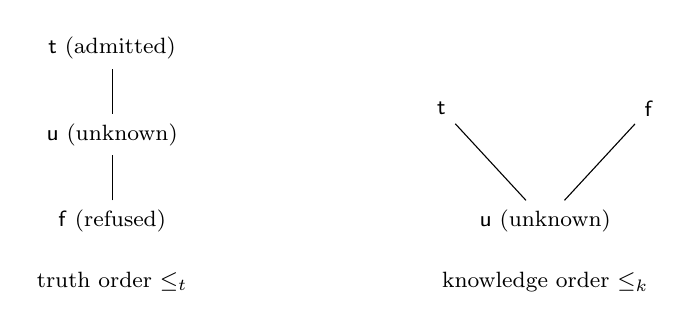
\begin{tikzpicture}[scale=1.1,every node/.style={font=\footnotesize}]
  % truth order (chain)
  \begin{scope}
    \node (f) at (0,0) {$\mathsf f$ (refused)};
    \node (u) at (0,1) {$\mathsf u$ (unknown)};
    \node (t) at (0,2) {$\mathsf t$ (admitted)};
    \draw (f)--(u)--(t);
    \node at (0,-0.7) {truth order $\le_t$};
  \end{scope}
  % knowledge order (V)
  \begin{scope}[xshift=5cm]
    \node (u2) at (0,0) {$\mathsf u$ (unknown)};
    \node (t2) at (-1.2,1.3) {$\mathsf t$};
    \node (f2) at (1.2,1.3) {$\mathsf f$};
    \draw (u2)--(t2); \draw (u2)--(f2);
    \node at (0,-0.7) {knowledge order $\le_k$};
  \end{scope}
\end{tikzpicture}
\caption[The two orders on three values]{The truth order $\le_t$ (a chain) and
the knowledge order $\le_k$ (unknown at the bottom; admitted and refused
incomparable above). \cref{prin:three-valued} is the statement that conformance
respects $\le_k$, in which \emph{unknown} is strictly below both polarities.}
\label{fig:k3}
\end{figure}

\begin{remark}[Belnap's four values]
Adding a fourth value $\top$ (\emph{both}, i.e.\ contradictory evidence) yields
Belnap's bilattice $\mathbf 4=\{\bot,\mathsf t,\mathsf f,\top\}$, a complete
lattice in the knowledge order with $\bot=\mathsf u$ at the bottom and $\top$ at
the top. The artifact's design \emph{refuses} $\top$: contradictory evidence is
surfaced as a \refused\ axis with a receipt rather than silently merged, which is
the A8/A9 ``tampering/anomaly'' discipline of \cref{tab:oracle}. We therefore
work in $\mathbf 3$ under $\le_k$, noting $\mathbf 4$ as the conservative
extension should contradiction ever need a first-class value.
\end{remark}

\subsection{The conformance lattice and the non-collapse theorem}
\label{sec:order-conformance}

\begin{definition}[Verdict assignment]
\label{def:verdict}
For a set $\mathcal A$ of law axes, a \emph{verdict assignment} is a function
$v\colon\mathcal A\to\mathbf 3$. The \code{ConformanceVector} is such a $v$
together with the induced partition
$\mathcal A=\admitted v\sqcup\refused v\sqcup\unknownstat v$ where
$\admitted v=v^{-1}(\mathsf t)$, etc.
\end{definition}

\begin{proposition}[Disjointness is functionality]
\label{prop:disjoint}
The three sets $\admitted v,\refused v,\unknownstat v$ are pairwise disjoint and
cover $\mathcal A$ if and only if $v$ is a (total) function. The bitmask
invariant of \cref{lst:cv} is exactly this functionality.
\end{proposition}
\begin{proof}
A function assigns each $a\in\mathcal A$ exactly one value, so its preimages
partition $\mathcal A$; conversely a partition into three labelled blocks defines
a unique value per element. The three disjoint bitmasks are the indicator vectors
of the blocks, and their pairwise disjointness with full coverage is the
single-valuedness and totality of $v$.
\end{proof}

Order the set of verdict assignments by the pointwise knowledge order:
$v\sqsubseteq w \iff \forall a.\ v(a)\le_k w(a)$. By
\cref{lem:product-lattice} this is a complete lattice with bottom
$\bot=\lambda a.\,\mathsf u$ (``all unknown'') and joins computed axiswise; the
join $v\sqcup w$ is defined unless some axis carries $\mathsf t$ in one and
$\mathsf f$ in the other, where it would require $\top$ (excluded above), marking
a genuine conflict.

\begin{definition}[Evidence refinement]
A step $v\sqsubseteq w$ is an \emph{evidence refinement}: on each axis the value
either is unchanged or moves up the knowledge order, i.e.\ $\mathsf u\to\mathsf t$
or $\mathsf u\to\mathsf f$. A move $\mathsf t\to\mathsf f$, $\mathsf f\to\mathsf
t$, $\mathsf t\to\mathsf u$, or $\mathsf f\to\mathsf u$ is \emph{not} a
refinement.
\end{definition}

\begin{theorem}[Non-collapse]
\label{thm:noncollapse}
Let $\Phi$ be the map taking an evidence state $E$ to its verdict assignment
$v_E$. If $\Phi$ is monotone from the evidence order to $(\,\cdot\,,\sqsubseteq)$,
then no axis can pass from $\mathsf u$ to $\mathsf t$ or to $\mathsf f$ without a
strict increase of evidence; in particular an \unknownstat\ axis is never
reported \admitted\ or \refused\ in the absence of new evidence.
\end{theorem}
\begin{proof}
Suppose axis $a$ has $v_E(a)=\mathsf u$ and $v_{E'}(a)\in\{\mathsf t,\mathsf f\}$
with $E'\not\sqsupset E$ in evidence. Since $\mathsf u<_k v_{E'}(a)$, we have
$v_E\not\sqsupseteq v_{E'}$ is consistent only if $v_E\sqsubset v_{E'}$, which by
monotonicity of $\Phi$ requires $E\sqsubset E'$, i.e.\ a strict evidence increase,
contradicting $E'\not\sqsupset E$. Hence no such collapse occurs.
\end{proof}

\Cref{thm:noncollapse} is \cref{prin:three-valued} proved, and its hypothesis
(monotonicity of $\Phi$) is exactly what the Oracle A11 check of
\cref{tab:oracle} enforces operationally: a transition $\unknownstat\to\{\admitted,\refused\}$
without a ``resolution event'' is flagged because it would witness a
non-monotone---hence evidence-free---collapse. Admissibility predicates inherit
the order:

\begin{corollary}[Monotonicity of release]
\label{cor:release}
The predicate $\mathrm{admits\text{-}release}(v)\equiv(\refused v=\varnothing)
\wedge(\neg\mathrm{strict}\vee\unknownstat v=\varnothing)$ of \cref{lst:cv} is
antitone in refusals and, under \code{strict\_mode}, antitone in unknowns: adding
a refusal or (in strict mode) an unknown can only revoke release, never grant it.
\end{corollary}
\begin{proof}
Immediate from the definition: enlarging $\refused v$ falsifies the first
conjunct; under strict mode, enlarging $\unknownstat v$ falsifies the second.
Neither enlargement can make a false conjunct true.
\end{proof}

\subsection{Scott continuity and conformance by replay}
\label{sec:order-scott}

Finally we connect the lattice to the artifact's \emph{replay} (\cref{sec:art-receipts}),
in which state is reconstructed from the receipt ledger. The right setting is
domain theory.

\begin{definition}[Dcpo and Scott continuity]
A \emph{directed-complete partial order} (dcpo) is a poset in which every directed
subset has a join. A map $f$ between dcpos is \emph{Scott-continuous} if it is
monotone and preserves directed joins: $f(\bigsqcup D)=\bigsqcup f(D)$.
\end{definition}

\begin{theorem}[Kleene least fixed point]
\label{thm:kleene-fix}
A Scott-continuous endomap $f$ on a pointed dcpo (one with a bottom $\bot$) has a
least fixed point $\mathrm{lfp}(f)=\bigsqcup_{n\in\mathbb N}f^{n}(\bot)$.
\end{theorem}
\begin{proof}
The chain $\bot\sqsubseteq f(\bot)\sqsubseteq f^2(\bot)\sqsubseteq\cdots$ is
directed; let $x=\bigsqcup_n f^n(\bot)$. By Scott continuity
$f(x)=\bigsqcup_n f^{n+1}(\bot)=x$, so $x$ is a fixed point. If $y=f(y)$ then
$\bot\sqsubseteq y$ gives $f^n(\bot)\sqsubseteq y$ by induction and monotonicity,
so $x\sqsubseteq y$; thus $x$ is least.
\end{proof}

\begin{proposition}[Conformance as a least fixed point]
\label{prop:replay-lfp}
Let $E\mapsto\mathrm{acc}(E)$ accumulate the evidence implied by replaying one
further receipt, and let $\Phi$ be Scott-continuous. Then the law-state obtained
by replaying the entire ledger from the all-unknown bottom is
$\Phi\bigl(\mathrm{lfp}(\mathrm{acc})\bigr)$, computed as the directed join of
finite replays.
\end{proposition}
\begin{proof}
Replaying receipts is iterating $\mathrm{acc}$ from $\bot$; the reachable evidence
is the directed join of the iterates, which by \cref{thm:kleene-fix} is
$\mathrm{lfp}(\mathrm{acc})$. Applying the Scott-continuous $\Phi$ commutes with
the join, giving the stated verdict.
\end{proof}

\Cref{prop:replay-lfp} is the order-theoretic reading of ``replay the log against
the model'': the law-state is not posited but \emph{constructed} as a least fixed
point of evidence accumulation, monotone by \cref{thm:noncollapse} and bottomed
at total ignorance. Conformance, in this artifact, begins from \unknownstat\ and
rises only on evidence---which is precisely the epistemic posture this thesis
adopts for its own claims (\cref{sec:m-epistemics}).
